\documentclass[a4paper,11pt]{article}
\usepackage[T1]{fontenc}
\usepackage[utf8]{inputenc}
\usepackage{lmodern}
\usepackage{hyperref}
\usepackage{graphicx}
\usepackage{rotating}

\title{Monetarily efficient Guass Elminiation given crappy hardware}
\author{Arash Rouhani and Jonas Ängeslevä}

\begin{document}

\maketitle

\section{Computer System}
We have written a gauss elimination program for MIPS assembler, the program is optimized for the hardware. Details below.
\subsection{hardware}
The MIPS processor have 5 pipe lines stages, seperate I and D cache, a write buffer and two coprocessors.
The caches can be in sizes of 128, 256 and 512 bytes, and are using LRU replacement policy and Write Back replacement policy.
The Least Recently Used is a replacement policy, where the element in the set that was least recently used is replaced, if the cache is full. Note that this only maters in N-way caches (where N>1).
The Write Back writing policy means that when writing to the memory, we don't actually write to the memory if the memory is cached. 
\subsection{software}
The algorithm used for the elimination is the one suggested.
Only some minor optimizations have been at an algorithmical level. We do not unncessisarily loop at the last row (it's always 0 0 ... 0 0 1).
This assumption makes our code to actually only work on invertable matrices.

For optimization, the code does use delayed branching slots, does not do indexing or call any subroutines. 
Furthermore it does not violate the MIPS conventions for subroutines, it however mutates a0, so the test program must be corrected accordingly.
\section{Configurations}
There are many ways to configure the hardware. We have experimentally tested and tabled some experiments, the parameters have been chosen to gradually try to increase the price*performence value, that is, we have used a \emph{greedily optimizing} method for parameter refining.

Changing the parameters sometimes give a significant effect, and sometimes it doesn't. If we look at the table, it's very clear that:
\begin{itemize}
\item An expensive I cache makes little difference.
\item 2-way associativity is superior. It outperforms 4 also in clock cycles.
\item Buffer size 1 is as fast as size 8 measured in clock cycles, but 1 is faster than 0.
\item The expensive memory outperforms the cheaper one from a price*performance standpoint.
In the rest of this subchapter we'll explain why we observe these extremities.
\end{itemize}
The I cache don't need to be big because the instructions are all close together, the whole content of the outermost loop definetly fits in 32 words, and we don't call subroutines, so the program pointer never leaves that scope.

One way associativity is bad because it doesn't play well with the data access patter.
See the Figure 4 in the assignment paper, there the (1) and (3) data accessor are rapidly sweeping lines.
(1) is sweeping the same line over and over again, we don't want (3) to throw out anything cached on the line where (1) is sweeping.
This is where two-way comes in, the competition for chache memory placement is decreased as two spots are available for every memory location.
Four way associativity however is to overhouse for the only 2 active sweepers.
Four-way associativity costs however, because searching in the cache must visit 4 locations, increasing delays.

A write buffer is not having a signifcant impacts, even though we do $O(n^3)$ writes.
Most writes are directly to cache memory rather than misses, so writing to real memory is often avoided, thus the need for a buffer decreased.

Reading from real memory however happens often, and that is why the expensive memory pays off.
This raises the question why it doesn't help to have a write buffer if memory interaction is common.
The reason is that most writes are to a memory location we've just read from, and therfor it is cached already.

%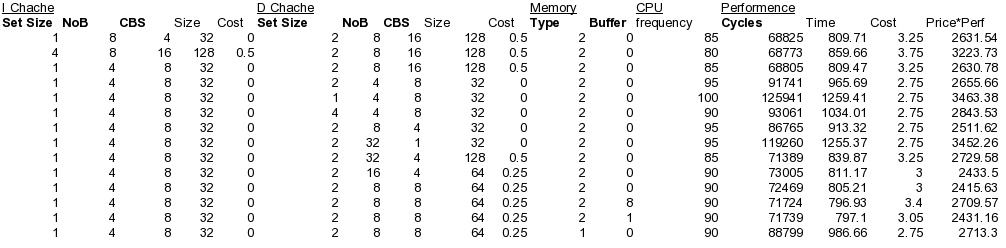
\includegraphics[width=210mm,height=297mm,angle=270]{table.png}
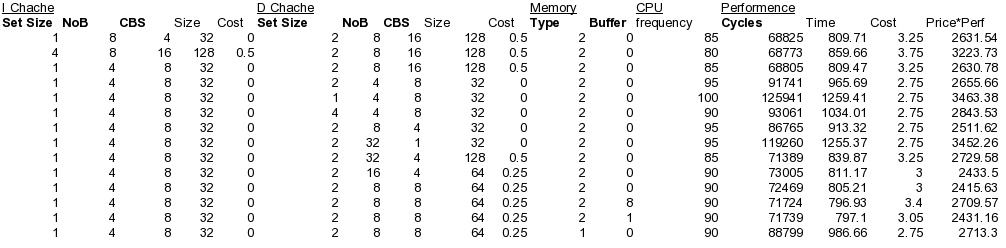
\includegraphics[angle=270]{table.png}

\end{document}
